\section{Exams 2023/24}
\subsection{June 2023}
\begin{exercise}
    Write the strong formulation of the initial-value problem under Dirichlet boundary conditions for the evolution Navier-Stokes equations in a smooth bounded domain $\Omega \subset \mathbb{R}^d$ with $d=2,3$. Then explain why the argument used for the proof of uniqueness of solution for \(n = 2\) cannot be extended to \(n = 3\).
\end{exercise}
First we write the strong formulation of evolutional Navier-Stokes equations
\begin{equation*}
    \begin{cases}
        \partial_t u - \nu \Delta u + (u \cdot \nabla)u + \nabla p = f, & \text{in } \Omega \times (0,T),          \\
        \nabla \cdot u = 0,                                             & \text{in } \Omega \times (0,T),          \\
        u = 0,                                                          & \text{on } \partial \Omega \times (0,T), \\
        u(\cdot,0) = u_0,                                               & \text{in } \Omega,
    \end{cases}
\end{equation*}

\begin{remark}[Weak formulation]
    We choose \(\bm{V}, \bm{H} = \bm{G_1}, \bm{V'}\). By choosing a test function \(v \in \bm{V}\), doing the usual integration by parts, and using the boundary condition, we obtain the weak formulation
    \begin{equation*}
        \text{Find } u \in \bm{L}^2(0,T;\bm{V}) \text{ s.t. }
        \begin{cases}
            \begin{aligned}
                \frac{d}{dt}(u(t), v)_H + \nu \int_\Omega \nabla u(t) : \nabla v \, dx + \\
                + \int_\Omega \left[ (u(t) \cdot \grad) u(t)\right] \cdot v \, dx = \langle f, v \rangle,
            \end{aligned} & \forall v \in \bm{V} \qquad \text{in } \mathcal{D}(0,T) \\
            u(0) = u_0.
        \end{cases}
    \end{equation*}
    This is the weakest possible formulation of the Navier-Stokes equations, we have no information on \(u\). We start with the least possible assumptions and we gain more informations step by step.
\end{remark}
For \(n=2\) we have global uniqueness for the solution, thanks to Ladyzhenskaya's inequality.
\begin{itemize}
    \item[\(n=2\)] We have the following inequality
          \[
              \norm{v}^2_{\bm{L}^4} \leq \sqrt{2} \norm{v}_{\bm{L}^2} \norm{\grad v}_{\bm{L}^2} \qquad \forall v \in \bm{H}^1_0(\Omega).
          \]
          This is an interpolation inequality: \(\bm{L}^4\) has a better regularity than
          \(\bm{L}^2\), but it is worse than \(\bm{H}^1\), so we can bound the
          \(\bm{L}^4\) norm with the \(\bm{H}^1\) and \(\bm{L}^2\) norms.
    \item[\(n=3\)] In this case Ladyzhenskaya's inequality states
          \[
              \norm{v}^2_{\bm{L}^4} \leq 2 \norm{v}_{\bm{L}^2}^{1/2} \norm{\grad v}_{\bm{L}^2}^{3/2} \qquad \forall v \in \bm{H}^1_0(\Omega).
          \]
          Due to Sobolev embeddings, increasing dimensions reduces the regularity of the
          solution. This inequality is not enough to prove uniqueness of the solution.
\end{itemize}
Since we know that if a solution satisfies \(u \in L^s(0,T;\bm{L}^r) \text{ with } \frac{2}{s}+\frac{n}{r} \leq 1\), then it is the unique solution. We can immediately see that for \(n=2\) we have \(s=4, r=4\), but increasing \(n\) breaks the inequality. This results means the we always have the existence of a solution, but only if we guarantee \(u \in L^s(0,T;\bm{L}^r)\) with the correct regularity we can have uniqueness.

\newpage
\begin{exercise}
    Consider the conservation law with two different initial conditions
    \begin{equation*}
        a)\,\begin{cases}
            u_t - \log(u) u_x = 0, & x \in \real, t > 0, \\
            u(x,0) = e^{-x},       & x \in \real,
        \end{cases}
        \qquad
        b)\,\begin{cases}
            u_t - \log(u) u_x = 0, & x \in \real, t > 0, \\
            u(x,0) = \begin{cases}
                         1, & x < 0,    \\
                         e, & x \geq 0.
                     \end{cases}
        \end{cases}
    \end{equation*}
    Discuss existence and uniqueness of classical and weak solutions for Cauchy problems. Then estabilish whether the found solutions satisfy the entropy condition.
\end{exercise}
\begin{remark}
    The problem, for a quasilinear partial differential equation,
    \[
        \left\{
        \begin{array}{ll}
            u_t + A(u) u_x = 0, & (x, t) \in \mathbb{R} \times \mathbb{R}_+ \\
            u(x, 0) = g(x),     & x \in \mathbb{R}
        \end{array}
        \right.
    \]
    is equavalent to the following parametric system of ordinary differential
    equations, where the parameter is \(x_0 \in \mathbb{R}\):
    \[
        \renewcommand{\arraystretch}{2.5}
        \left\{
        \begin{array}{ll}

            \frac{dt}{ds} = 1,    & t(0) = 0      \\
            \frac{dx}{ds} = A(u), & x(0) = x_0    \\
            \frac{du}{ds} = 0,    & u(0) = g(x_0)
        \end{array}
        \right.
        \quad \Rightarrow \quad
        \renewcommand{\arraystretch}{1.5}
        \left\{
        \begin{array}{l}
            t = s + 0       \\
            x = A(u)s + x_0 \\
            u = g(x_0)
        \end{array}
        \right.
    \]
    So the characteristic lines at \(x_0\) are given by \[x(t) = x_0 + A(g(x_0))t\] and the solution is constant along the characteristics. For those interested in
    understanding (briefly) more generally the method of characteristics for
    quasilinear equations, a more detailed discussion can be found in Chapter 2.2
    of the \href{https://github.com/alessandropedone/cauchy-kowalevski-theorem}
    {\textcolor{blue}{Bachelor's thesis of one of the contributors}}.
\end{remark}

\begin{itemize}
    \item[\textbf{a)}]
          In this case we have that \(A(u) = -\log(u)\) and \(g(x) = e^{-x}\).
          So the characteristic lines are given by
          \[
              x(t) = x_0 - \log(e^{-x_0})t = x_0 + x_0 t
          \]
          And now we want to find the solution u along the characteristics. Since u is
          constant along the characteristics, we search the point \((x0,0)\) such that
          the corresponding characteristic line passes through \((x,t)\):
          \[
              x_0 + x_0 t = x \quad \Rightarrow \quad x_0 = \frac{x}{1+t}.
          \]
          The solution is then:
          \[
              u(x,t) = g\left(\frac{x}{1+t}\right) = e^{-\frac{x}{1+t}}.
          \]
          This is a classical global solution belonging to \(C^1(\real \times (0,
          \infty))\), and thanks to the method of characteristics we have uniqueness. A
          classical solution is also a weak solution. Moreover, the solution satisfies
          the entropy condition, since
          \[
              u(x+a,t)-u(x,t) = e^{-\frac{x+a}{1+t}} - e^{-\frac{x}{1+t}} = e^{-\frac{x}{1+t}} \underbrace{\left(e^{-\frac{a}{1+t}}-1\right)}_{\leq 0} \leq 0 \leq \frac{Ea}{t}.
          \]
    \item[\textbf{b)}]
          In this case we have that \(A(u) = -\log(u)\) and \[g(x) = \begin{cases}
                  1, & x < 0, \\
                  e, & x > 0.
              \end{cases}\]
          The characteristics are given by
          \[
              x(t) = x_0 - \log(g(x_0))t = \begin{cases}
                  x_0,      & x_0 < 0 \\
                  -t + x_0, & x_0 > 0
              \end{cases}
          \]
          And now we want to find the solution $u$ along the characteristics. Since $u$
          is constant along the characteristics, we search the point \((x_0,0)\) such
          that the corresponding characteristic line passes through \((x,t)\). For
          example we have that
          \[
              x_0 - \log(g(x_0))t = x \quad \Rightarrow \quad x_0 = \begin{cases}
                  x,      & x < 0, \\
                  -t + x, & x > 0.
              \end{cases}
          \]
          But this is not the only possible choice. The solution is then:
          \[
              u(x,t) = \begin{cases}
                  1  & x < 0 \\
                  e, & x > 0
              \end{cases}
          \]
          This cannot be a classical solution, since it is not differentiable at \(x=0\).
          And it is not a weak solution since it doesn't satisfy the jump condition (Rankine-Hugoniot), as
          we will see in a moment. Infact, to compute the shock speed, we define and
          compute
          \[B(u) = \int_0^u A(s) \, ds = u - u \log(u).\]
          So we obtain that
          \[
              \eta'(t) = \frac{[B(u)]}{[u]} = \frac{B(u_+)- B(u_-)}{u_+-u_-} = \frac{(e - e \log(e)) - (1 - 1 \log(1))}{e - 1} = \frac{1}{1-e}.
          \]
          So can we represent this in the \((x,t)\) plane as follows:
          \begin{center}
              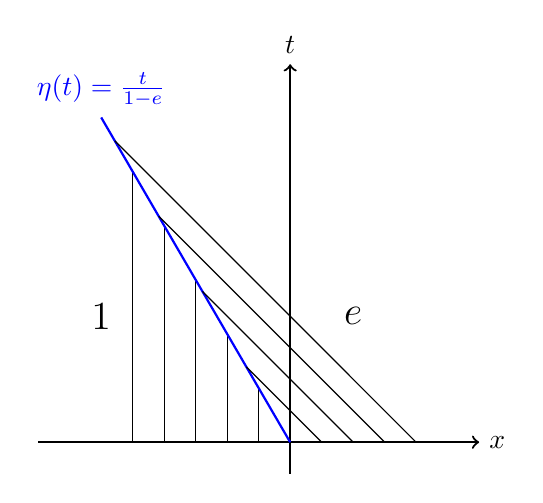
\begin{tikzpicture}[scale=0.8]

                  % Draw axes
                  \draw[thick, ->] (-4,0) -- (3,0) node[right] {$x$};
                  \draw[thick, ->] (0,-0.5) -- (0,6) node[above] {$t$};

                  % Vertical lines when x_0 < 0
                  \draw (-2.5,0) -- (-2.5,2.5/0.582);
                  \draw (-2,0) -- (-2,2/0.582);
                  \draw (-1.5,0) -- (-1.5,1.5/0.582);
                  \draw (-1,0) -- (-1,1/0.582);
                  \draw (-0.5,0) -- (-0.5,0.5/0.582);

                  % Function η(t) = t/(1-e) ≈ t/(-1.718) ≈ -0.582t
                  % Draw this as a function of x (treating x as t)
                  \draw[thick, blue] (0,0) -- (-3,3/0.582) node[above] {$\eta(t) = \frac{t}{1-e}$};

                  % Line x = -t + 1 when x_0 > 0, rearranged as t = -x + x_0
                  % Extended to meet the blue line
                  \pgfmathdeclarefunction{f}{1}{%
                      \pgfmathparse{#1/(1-0.582)}
                  }
                  \draw (0.5,0) -- ({(-0.582)*f(0.5)}, {f(0.5)});
                  \draw (1,0) -- ({(-0.582)*f(1)}, {f(1)});
                  \draw (1.5,0) -- ({(-0.582)*f(1.5)}, {f(1.5)});
                  \draw (2,0) -- ({(-0.582)*f(2)}, {f(2)});

                  % Add region labels
                  % Region to the left of the blue line (where solution = 1)
                  \node at (-3, 2) {\Large $1$};

                  % Region to the right of the blue line (where solution = e)
                  \node at (1, 2) {\Large $e$};
              \end{tikzpicture}
          \end{center}
          In the end, the only weak solution, i.e. the only solution the does satisfy the jump condition,
          to this problem is
          \[
              u(x,t) = \begin{cases}
                  1  & x < \eta(t) \\
                  e, & x > \eta(t)
              \end{cases}
          \]
          Now it's easy to check that the entropy condition is not satisfied, since for
          any \(E>0\) and \(a > 0\) we can find a couple of points \(x\) and \(t\) such
          that
          \[
              \underbrace{u(x+a,t)}_{=e} - \underbrace{u(x,t)}_{=1} > \frac{Ea}{t}.
          \]
          The idea is just to take \((x, t)\) such that \(x + a > \eta(t)\) and \(x <
          \eta(t)\) and \(t\) big enough to make sure that $e-1>Ea/t$.
\end{itemize}

\newpage
\begin{exercise}
    Let \(\Omega \subset \real^3\) be a bounded Lipschitz domain. Prove that the problem
    \begin{equation*}
        \begin{cases}
            \grad \cdot u = 0, & \text{in } \Omega,          \\
            u  = 0,            & \text{on } \partial \Omega,
        \end{cases}
    \end{equation*}
    has infinitely many solutions in \(C^\infty(\Omega) \cap C^0(\overline{\Omega})\).
\end{exercise}
We can prove this with the help of Helmoltz decomposition. We can write any vector field \(u\) as the sum of a solenoidal and an irrotational part
\[
    u = \grad \phi + \grad \times \psi.
\]
where \(\phi\) is the scalar potential and \(\psi\) is the vector potential.
Our constraint is that the divergence of \(u\) is zero, so we have
\[
    \grad \cdot u = \grad \cdot \grad \phi + \grad \cdot \grad \times \psi = \Delta \phi = 0 \quad \Rightarrow \quad \grad \phi = \text{const.}
\]
This means that the scalar potential is constant and we can rewrite the
decomposition
\[
    u = \grad \phi + \grad \times \psi = \grad \times \psi + C
\]
Now, choosing \(\psi\) such that satisfies the boundary condition, we can have
infinitely many solutions, since
\[
    \grad \cdot u = \grad \cdot \grad \times \psi + \grad \cdot C = 0 \quad \forall \psi \in  C^\infty(\Omega) \cap C^0(\overline{\Omega}).
\]

\newpage
\begin{exercise}
    Let \(\Omega \subset \real^n\) be a smooth bounded open set. Prove that the problem
    \begin{equation*}
        \begin{cases}
            \Delta u = u^3, & \text{in } \Omega,          \\
            u = 0,          & \text{on } \partial \Omega,
        \end{cases}
    \end{equation*}
    admits a unique classical solution and determine it.
\end{exercise}
We can prove the uniqueness of the solution by using the energy method. We multiply the equation by \(u\) and integrate over \(\Omega\)
\[
    \int_\Omega u \Delta u \, dx = \int_\Omega u^4 \, dx.
\]
Using the divergence theorem we have
\[
    -\int_\Omega \abs{\grad u}^2 \, dx = \int_\Omega u^4 \, dx.
\]
We have that the left side is negative, while the right side is positive, so
the only way to have a solution is to have \(u = 0\). This is the unique
solution to the problem.

\newpage
\subsection{July 2023}
\begin{exercise}
    Consider the two second order sobolev spaces \(H^2_0(-1, 1)\) and \(H^2(-1, 1) \cap H^1_0(-1, 1)\).
    \begin{enumerate}
        \item Prove that the map
              \[
                  (u, v) \longmapsto \int_{-1}^1 \left[ u''(x) v''(x) + u'(x) v'(x) + u(x) v(x) \right] \, dx
              \]
              defines a scalar product that turns both Sobolev spaces into Hilbert spaces.
        \item Prove that the map
              \[
                  (u, v) \longmapsto \int_{-1}^1 u''(x) v''(x) \, dx
                  \tag{(M)}
              \]
              defines a scalar product that turns both Sobolev spaces into Hilbert spaces.
        \item Determine a basis of the orthogonal complement of \(H^2_0(-1, 1)\) into
              \(H^2(-1, 1)\cap H^1_0(-1, 1)\) with respect to the scalar product \((M)\).
    \end{enumerate}
\end{exercise}
We start by checking the properties of the scalar product
\begin{remark}
    Let \(X\) be a vector space and we define a function
    \[
        \begin{aligned}
            \langle \cdot, \cdot \rangle : X \times X & \longrightarrow \real            \\
            (u, v)                                    & \longmapsto \langle u, v \rangle
        \end{aligned}
    \]
    such that for all \(u, v, w \in X\) and \(\alpha \in \real\) we have
    \begin{enumerate}
        \item \(\langle u, u \rangle \leq 0\), and \(\langle u, u \rangle = 0 \iff u = 0\) (non-degeneracy),
        \item \(\langle u, v \rangle = \langle v, u \rangle\) (symmetry),
        \item \(\langle \alpha u + \beta v, w \rangle = \alpha \langle u, w \rangle + \beta \langle v, w \rangle\) (linearity),
    \end{enumerate}
    then \(\langle \cdot, \cdot \rangle\) is a scalar product.
\end{remark}
Now we check if the given scalar products satisfy the properties.
\begin{enumerate}
    \item Starting with the first one
          \[
              \begin{aligned}
                  \langle u, u \rangle & = \int_{-1}^1 \left[ u''(x)^2 + u'(x)^2 + u(x)^2 \right] \, dx \geq 0, \\
                  \langle u, u \rangle & = 0 \iff u''(x) = u'(x) = u(x) = 0 \quad \forall x \in (-1, 1).
              \end{aligned}
          \]
          is true because in the first case is the sum of squares, and in the second case
          we have that \(u = 0\) means that all its derivatives are zero.

          For the symmetry property we see that is defined as sum of products, so it is
          symmetric.

          Then we check the linearity
          \[
              \begin{aligned}
                  \langle \alpha u + \beta v, w \rangle & = \int_{-1}^1 \left[ (\alpha u + \beta v)''(x) w''(x) + (\alpha u + \beta v)'(x) w'(x) + (\alpha u + \beta v)(x) w(x) \right] \, dx \\
                                                        & = \alpha \int_{-1}^1 \left[ u''(x) w''(x) + u'(x) w'(x) + u(x) w(x) \right] \, dx +                                                 \\
                                                        & + \beta \int_{-1}^1 \left[ v''(x) w''(x) + v'(x) w'(x) + v(x) w(x) \right] \, dx                                                    \\
                                                        & = \alpha \langle u, w \rangle + \beta \langle v, w \rangle.
              \end{aligned}
          \]
          This is true because derivatives and integrals are linear operators, and we can
          say that this map defines a scalar product. Now we need to check that the
          induced norm is complete, meaning that each Cauchy sequence converges. We have
          the norm
          \[
              \norm{u}_* = \sqrt{\langle u, u \rangle} = \sqrt{\int_{-1}^1 \left[ u''(x)^2 + u'(x)^2 + u(x)^2 \right] \, dx}.
          \]
          The standard norm in \(H^2_0(-1, 1)\) is
          \[
              \norm{u}_{H^2_0} = \sqrt{\int_{-1}^1 u''(x)^2 \, dx}.
          \]
          We can see that the two norms are equivalent, starting with the inequality
          \begin{align*}
              \norm{u}_{H^2_0} & \leq \norm{u}_*
          \end{align*}
          we only need to prove the opposite inequality. We start from \(\int_{-1}^1 -u''(x) u (x) \, dx \) and obtain
          \[
              \begin{split}
                  \frac{1}{2} \norm{u''(x)}^2_{L^2} + \frac{1}{2} \norm{u}^2_{L^2} = \int_{-1}^1 \frac{u''(x)^2}{2} + \frac{u(x)^2}{2} \, dx \geq \int_{-1}^1 u''(x) u(x) \, dx = \\= \int_{-1}^1 u'(x) u'(x) \, dx - \cancel{\left. u'(x) u(x) \right|_{-1}^1} = \norm{u'}^2_{L^2}.
              \end{split}
          \]
          Since by Poincaré inequality we have that \(\norm{u}_{L^2} \leq C
          \norm{u''}_{L^2}\), we have that \(\norm{u'}_{L^2}^2 \leq C
          \norm{u''}_{L^2}^2\), and also \(\norm{u}_{L^2}^2 \leq C \norm{u''}_{L^2}^2\).
          This means
          \[
              \norm{u}_{L^2}^2 + \norm{u'}_{L^2}^2 + \norm{u''}_{L^2}^2 \leq C \norm{u''}_{L^2}^2 \quad \Rightarrow \quad \norm{u}_* \leq C \norm{u}_{H^2_0}.
          \]
          This means that the two norms are equivalent, and since \(H^2_0(-1, 1)\) is
          complete, also the space defined by the scalar product is complete.

          Now we do the same proof for the space \(H^2(-1, 1) \cap H^1_0(-1, 1)\). We
          have the norm
          \[
              \norm{u}_* = \sqrt{\int_{-1}^1 \left[ u''(x)^2 + u'(x)^2 + u(x)^2 \right] \, dx}.
          \]
          The standard norm in \(H^2(-1, 1) \cap H^1_0(-1, 1)\) is
          \[
              \norm{u}_{H^2} = \sqrt{\int_{-1}^1 u''(x)^2 + u'(x)^2 \, dx}.
          \]
          We can clearly see that
          \[
              \norm{u}_{H^2} \leq \norm{u}_* \leq C \norm{u}_{H^2}.
          \]
          Now let's prove the othe inequality. by Poincaré inequality we have that
          \(\norm{u}_{L^2} \leq C \norm{u''}_{L^2}\), so we have the same reasoning as
          before.
    \item For the second scalar product we have
          \[
              \begin{aligned}
                  \langle u, u \rangle & = \int_{-1}^1 u''(x)^2 \, dx \geq 0,             \\
                  \langle u, u \rangle & = 0 \iff u''(x) = 0 \quad \forall x \in (-1, 1).
              \end{aligned}
          \]
          Same reasoning as before, also for the symmetry and linearity properties, so
          also this map defines a scalar product. Now we need to check that the induced
          norm is complete, meaning that each Cauchy sequence converges. For the first
          space \(H^2_0(-1, 1)\) we have the norm is already the standard norm, so the
          space is complete. For the second space \(H^2(-1, 1) \cap H^1_0(-1, 1)\) we
          have the norm
          \[
              \norm{u}_* = \sqrt{\int_{-1}^1 u''(x)^2 \, dx}.
          \]
          complies with the inequality
          \[
              \norm{u}_* \leq \norm{u}_{H^2\cap H^1_0}.
          \]
          To check the opposite inequality we start from \(\int_{-1}^1 -u''(x) u (x) \,
          dx \) and obtain
          \[
              \begin{split}
                  \frac{1}{2} \norm{u''(x)}^2_{L^2} + \frac{1}{2} \norm{u}^2_{L^2} = \int_{-1}^1 \frac{u''(x)^2}{2} + \frac{u(x)^2}{2} \, dx \geq \int_{-1}^1 u''(x) u(x) \, dx = \\= \int_{-1}^1 u'(x) u'(x) \, dx - \cancel{\left. u'(x) u(x) \right|_{-1}^1} = \norm{u'}^2_{L^2}.
              \end{split}
          \]
          So we have that \(\norm{u''}_{L^2}^2 \geq \norm{u'}_{L^2}^2\). Since
          \[
              \norm{u}_{H^2}^2 = \norm{u''}_{L^2}^2 + \norm{u'}_{L^2}^2 \leq C \norm{u''}_{L^2}^2 = C \norm{u}_*^2
          \]

    \item We now need to determine a basis of the orthogonal complement of \(H^2_0(-1,
          1)\) into \(H^2(-1, 1)\cap H^1_0(-1, 1)\) with respect to the scalar product
          \((M)\). To do so, we need to find all the functions \(v \in H^2_0(-1, 1)\)
          such that
          \[
              \int_{-1}^1 u''(x) v''(x) \, dx = 0 \quad \forall u \in H^2(-1, 1)\cap H^1_0(-1, 1).
          \]
          Integrating by parts we have
          \[
              \int_{-1}^1 u''(x) v''(x) \, dx = \cancel{\left. v'(x) u''(x) \right|_{-1}^1} - \int_{-1}^1 u'''(x) v'(x) \, dx = 0.
          \]
          Again integrating by parts we have
          \[
              -\int_{-1}^1 u'''(x) v'(x) \, dx = -\cancel{\left. v(x) u'''(x) \right|_{-1}^1} + \int_{-1}^1 u''''(x) v(x) \, dx = 0.
          \]
          So we have obtained
          \[
              \int_{-1}^1 u''''(x) v(x) \, dx = 0 \quad \forall u \in H^2(-1, 1)\cap H^1_0(-1, 1).
          \]
          Which is the weak formulation of the problem
          \[
              \begin{cases}
                  u''''(x) = 0, & \text{in } (-1, 1),          \\
                  u = 0         & \text{on } \partial (-1, 1).
              \end{cases}
          \]
          The general solution of this problem is
          \[
              u(x) = a + bx + cx^2 + d x^3.
          \]
          Since we have the boundary condition \(u(1) = u(-1) = 0\) we have that
          \[
              \begin{cases}
                  a + b + c + d = 0, \\
                  a - b + c - d = 0.
              \end{cases}
          \]
          Solving this gives us \(b = -d\) and \(a = -c\), so the general solution is
          \[
              u(x) = c(x^2 - 1) + d(x^3 - x).
          \]
          and the basis of the orthogonal complement is given by
          \[
              \left\{ x^2 - 1, x^3 - x \right\}.
          \]
\end{enumerate}

\newpage
\begin{exercise}
    Write the weak formulation of the forced stationary Navier-Stokes equations under Dirichlet boundary conditions in a smooth bounded domain \(\Omega \subset \real^n\) and explain why the assumption \(n \leq 4\) is needed.
\end{exercise}
We start by writing the stationary Navier-Stokes equations
\[
    \begin{cases}
        - \eta \Delta u + \left( u \cdot \grad \right) u + \grad p = f & \Omega         \\
        \div u = 0                                                     & \Omega         \\
        u = 0                                                          & \partial\Omega
    \end{cases}
\]
where \(\Omega \subset \real^n\), \(\partial\Omega \in C^1\), and \(n \leq 4\).
\begin{remark}
    About the term \(\left( u \cdot \grad \right) u\), we have that (\(n = 3\))
    \[
        u = \begin{pmatrix}
            u_1 \\
            u_2 \\
            u_3
        \end{pmatrix} \quad \text{and} \quad \grad = \begin{pmatrix}
            \partial_1 \\
            \partial_2 \\
            \partial_3
        \end{pmatrix}
    \]
    So combining the two we have
    \[
        \begin{split}
            \left( u \cdot \grad \right) u = \begin{pmatrix}
                                                 u_1 \partial_1 + u_2 \partial_2 + u_3 \partial_3
                                             \end{pmatrix} \begin{pmatrix}
                                                               u_1 \\
                                                               u_2 \\
                                                               u_3
                                                           \end{pmatrix} = \begin{pmatrix}
                                                                               u_1 \partial_1 u_1 + u_2 \partial_2 u_1 + u_3 \partial_3 u_1 \\
                                                                               u_1 \partial_1 u_2 + u_2 \partial_2
                                                                               u_2 + u_3 \partial_3 u_2                                     \\
                                                                               u_1 \partial_1 u_3 + u_2 \partial_2 u_3 + u_3 \partial_3 u_3
                                                                           \end{pmatrix}
        \end{split}
    \]
    which is the so-called convective term.
\end{remark}
As functional spaces we choose the spaces introduced in the previous exercise about the Stokes problem \(\bm{V}, \bm{G_1}, \bm{G_2}, \bm{G_3}\).
\begin{remark}
    \(\bm{V} \coloneqq \left\{ f \in \bm{H}^1_0(\Omega) \mid \grad \cdot f = 0 \right\}\) is the space of divergence-free functions.
    We also introduce three spaces:
    \begin{itemize}
        \item \(\bm{G}_1 \coloneqq \left\{ f \in \bm{L}^2(\Omega) \mid \grad \cdot f = 0, \gamma_\nu f = 0 \right\}\)
        \item \(\bm{G}_2 \coloneqq \left\{ f \in \bm{L}^2(\Omega) \mid \grad \cdot f = 0, \exists g \in H^1(\Omega) \text{ s.t. } f = \grad g \right\}\)
        \item \(\bm{G}_3 \coloneqq \left\{ f \in \bm{L}^2(\Omega) \mid \exists g \in H^1_0(\Omega) \text{ s.t. } f = \grad g \right\}\)
    \end{itemize}
\end{remark}
We now multiply the equation by a test function \(v \in \bm{V}\) and obtain
\[
    \begin{split}
        - \eta \int_\Omega \Delta u v \, dx + \int_\Omega \left( u \cdot \grad \right) u v \, dx + \int_\Omega \grad p \cdot v \, dx = \int_\Omega f v \, dx
    \end{split}
\]
We integrate by parts the first term and obtain
\[
    \begin{split}
        \eta \int_\Omega \grad u : \grad v \, dx + \int_\Omega \left( u \cdot \grad \right) u \cdot v \, dx + \underbrace{\int_\Omega \grad p \cdot v \, dx}_{=0} = \int_\Omega f v \, dx
    \end{split}
\]
The term \(\int_\Omega \grad p v \, dx\) is zero because \(v \in \bm{V}
\subseteq \bm{G_1}\) and \(\grad p \in \bm{G_2} \oplus \bm{G_3} =
\bm{G_1}^\perp\). We can now write the weak formulation of the problem
\[
    \begin{split}
        \text{Find } u \in \bm{V} \text{ such that } \eta \int_\Omega \grad u : \grad v \, dx + \int_\Omega \left( u \cdot \grad \right) u \cdot v \, dx = \langle f, v \rangle \qquad \forall v \in \bm{V}
    \end{split}
\]
Now we need to explain why the assumption \(n \leq 4\) is necessary. We need to
understand in which space the convective term lies and that \(v \in \bm{V}
\Rightarrow \grad v \in \bm{L}^2(\Omega)\).
\begin{itemize}
    \item[\(n = 2\)] In the bidimensional case, we have that \(u \in \bm{V} \Rightarrow u \in \bm{L}^p(\Omega) \, \forall 1 \leq p < \infty\). Since \(u \cdot \grad u\) is a product of a function in \(\bm{L}^p(\Omega)\) and a function in \(\bm{L}^2(\Omega)\), we have that \(u \cdot \grad u \in \bm{L}^2(\Omega) \, \forall q < 2\).
          \[
              \begin{pmatrix*}
                  \bm{H}^1_0(\Omega) \subset \bm{L}^p{(\Omega)} & \forall 1 \leq p < \infty \\
                  \bm{L}^{p'}(\Omega) \subset \bm{H}^{-1}(\Omega) & \forall 1 < p \leq \infty
              \end{pmatrix*}
              \Rightarrow u \cdot \grad u \in \bm{H}^{-1}(\Omega)
          \]
    \item[\(n = 3\)] In the tridimensional case, Sobolev embedding gives us \(u \in \bm{V} \Rightarrow u \in \bm{L}^6(\Omega)\). In this case we have that \(u \cdot \grad u \in \bm{L}^{3/2}(\Omega)\), because we have that \(u \in \bm{L}^6(\Omega)\) and \(\grad u \in \bm{L}^2(\Omega)\), and by Holder's inequality \(\frac{1}{6} + \frac{1}{2} + \frac{1}{r} = 1 \Rightarrow r = 3\) and the dual of \(\bm{L}^{3}(\Omega)\) is \(\bm{L}^{3/2}(\Omega)\).
          \[
              \begin{pmatrix*}
                  \bm{H}^1_0(\Omega) \subset \bm{L}^6{(\Omega)}  \\
                  \bm{L}^{6/5}(\Omega) \subset \bm{H}^{-1}(\Omega)
              \end{pmatrix*}
              \Rightarrow u \cdot \grad u \in \bm{L}^{3/2}(\Omega) \subset \bm{L}^{6/5}(\Omega) \subset \bm{H}^{-1}(\Omega)
          \]
    \item[\(n = 4\)] In the four-dimensional case, we have that \(u \in \bm{V} \Rightarrow u \in \bm{L}^4(\Omega)\). In this case we have that \(u \cdot \grad u \in \bm{L}^{4/3}(\Omega)\), because we have that \(u \in \bm{L}^4(\Omega)\) and \(\grad u \in \bm{L}^2(\Omega)\), and by Holder's inequality \(\frac{1}{4} + \frac{1}{2} + \frac{1}{r} = 1 \Rightarrow r = 4\) and the dual of \(\bm{L}^{4}(\Omega)\) is \(\bm{L}^{4/3}(\Omega)\).
          \[
              \begin{pmatrix*}
                  \bm{H}^1_0(\Omega) \subset \bm{L}^4{(\Omega)}  \\
                  \bm{L}^{4/3}(\Omega) \subset \bm{H}^{-1}(\Omega)
              \end{pmatrix*}
              \Rightarrow u \cdot \grad u \in \bm{H}^{-1}(\Omega)
          \]
    \item[\(n = 5\)] In the five-dimensional case, we have that \(u \in \bm{V} \Rightarrow u \in \bm{L}^{10/3}(\Omega)\). In this case we have that \(u \cdot \grad u \in \bm{L}^{5/4}(\Omega)\), because we have that \(u \in \bm{L}^{10/3}(\Omega)\) and \(\grad u \in \bm{L}^2(\Omega)\), and by Holder's inequality \(\frac{3}{10} + \frac{1}{2} + \frac{1}{r} = 1 \Rightarrow r = 5\) and the dual of \(\bm{L}^{5}(\Omega)\) is \(\bm{L}^{5/4}(\Omega)\).
          \[
              \begin{pmatrix*}
                  \bm{H}^1_0(\Omega) \subset \bm{L}^{10/3}{(\Omega)}  \\
                  \bm{L}^{10/7}(\Omega) \subset \bm{H}^{-1}(\Omega)
              \end{pmatrix*}
              \nRightarrow u \cdot \grad u \in \bm{L}^{10/7}(\Omega) \subset \bm{H}^{-1}(\Omega) \text{ because } \frac{5}{4} < \frac{10}{7}
          \]
          Because \(L^q \subset L^p\) if \(p < q\), in \(n = 5\) we do not have that \(u
          \cdot \grad u \in \bm{H}^{-1}(\Omega)\).
\end{itemize}

\newpage
\begin{exercise}
    It is known that if \(w(\cdot, t) \in \mathcal{S}(\real)\) satisfies \(w_t + 6(w - \epsilon w^2)w_x + w_{xxx} = 0\) in \(\real \times \real^+\), then, for all \(\epsilon \geq 0\),
    the function \(u \coloneqq w + \epsilon w_x - \epsilon^2 w^2\) satisfies the Korteweg-de Vries equation
    \[
        u_t + 6uu_x + u_{xxx} = 0 \quad \text{in } \real \times \real^+.
    \]
    Prove that the Korteweg-de Vries equation has infinitely many conserved
    quantities.
\end{exercise}
We will add the assumptions that we know that mass and momentum, and energy are conserved for the KdV equation.
To prove this, we start by rewriting the equation in \(w\) as
\[
    w_t + \left(3w^2 - 2\epsilon^2 w^3\right)_x + \left(w_{xx}\right)_x = 0 \Rightarrow u \text{ solves KdV } \Rightarrow \int w \text{ is conserved for all } \epsilon \geq 0.
\]
Then we write \(w = w(x, t; \epsilon)\) to highlight the dependence on
\(\epsilon\). It can be proved that this dependence \(\epsilon \mapsto w(x, t;
\epsilon)\) is analytic, so we can write
\[
    w(x, t; \epsilon) = \sum_{n=0}^\infty \epsilon^n w_n(x, t).
\]
which is the power series expansion of \(w\) in \(\epsilon\), and \(
\frac{d}{dt} \int w_n \, dx = 0 \text{ because mass is conserved.} \) At this
point we rewrite \(u\) as
\begin{align*}
    u & = w + \epsilon w_x - \epsilon^2 w^2 =                                                                                                            \\
      & = \sum_{n=0}^\infty \epsilon^n w_n + \sum_{n=0}^\infty \epsilon^{n+1} (w_{n})_x - \sum_{n=0}^\infty \epsilon^{n+2} w_n^2 =                       \\
      & = w_0 + \epsilon \left[w_1 + (w_0)_x\right] + \epsilon^2 \left[w_2 + (w_1)_x - w_0^2\right] + \epsilon^3 \left[w_3 + (w_2)_x - 2w_0 w_1\right] + \\
      & + \epsilon^4 \left[w_4 + (w_3)_x - 2w_0 w_2 - w_1^2\right] + R_4(\epsilon).
\end{align*}
Where in the last step we used the MacLaurin expansion in term of \(\epsilon\). But \(u\) has no dependence on \(\epsilon\), so we have that \((\cdot)\epsilon^n = 0\) for all \(n\).
\begin{align*}
     & w_0 = u,                                                                    \\
     & w_1 + (w_0)_x = -(w_0)_x = -u_x,                                            \\
     & w_2 + (w_1)_x - w_0^2 = u^2 - u_{xx},                                       \\
     & w_3 + (w_2)_x - 2w_0 w_1 = -u_{xxx} - 4uu_x,                                \\
     & w_4 + (w_3)_x - 2w_0 w_2 - w_1^2 = 5 u_x^2 + 6 u u_{xx} + u_{xxxx} + 2 u^3.
\end{align*}
Now we integrate all the equations in \(x\) and we obtain
\begin{align*}
    \int w_0 \, dx & = \int u \, dx = 0, \text{ mass}                                                                               \\
    \int w_1 \, dx & = -\underbrace{\int u_x \, dx}_{\text{\tiny div. form}} = 0, \text{ conserved}                                 \\
    \int w_2 \, dx & = \int u^2 \, dx - \int u_{xx} \, dx = \int u^2 \, dx, \text{ momentum}                                        \\
    \int w_3 \, dx & = -\int u_{xxx} \, dx - 4 \int u u_x \, dx = - \int \left(2 u^2 + u_{xx}\right)_x \, dx = 0, \text{ conserved} \\
    \int w_4 \, dx & = 5 \int u_x^2 \, dx + 6 \int u u_{xx} \, dx + \int u_{xxxx} \, dx + 2 \int u^3 \, dx =                        \\
                   & \underset{\mathclap{\text{IPP}}}{=} \int \left(2 u^3 - u_x^2\right) \, dx = 0, \text{ energy}.
\end{align*}
We find infinitely many conserved quantities for the KdV equation, with an increasing power of \(u\).

\newpage
\subsection{September 2023}
\begin{exercise}
    Let \(\Omega \subset \real^2\) be a bounded open set of class \(C^1\), and let \(f \in L^2(\Omega)\). Consider the Dirichlet problem
    \begin{equation*}
        \begin{cases}
            u_{tt} - \left(\partial_x^2 u + 2 \partial_y^2 u - 2 \partial_{xy} u\right) = f, & \text{in } \Omega \times (0, T),          \\
            u = 0,                                                                           & \text{on } \partial \Omega \times (0, T), \\
            u(x,0) = u_0(x),                                                                 & x \in \Omega,                             \\
            u_t(x,0) = u_1(x),                                                               & x \in \Omega.
        \end{cases}
        \tag{(P)}
    \end{equation*}
    \begin{enumerate}
        \item For a suitable symmetric matrix \(A\), write the PDE appearing in (P) in the
              form \(u_{tt} - \div(A \grad u) = f\).
        \item Write the weak formulation of (P).
        \item Sketch the proof of existence and uniqueness of a solution of (P), explaining
              to which functional spaces is expected to belong.
    \end{enumerate}
\end{exercise}
\begin{enumerate}
    \item We start by writing the PDE in the form \(u_{tt} - \div(A \grad u) = f\). We
          have that
          \[
              u_{tt} - \left(A_{11} u_{xx} + A_{22} u_{yy} + 2A_{12} u_{xy}\right) = f.
          \]
          We can write the matrix \(A\) as
          \[
              A = \begin{pmatrix}
                  2  & -1 \\
                  -1 & 2
              \end{pmatrix}
          \]
          and the PDE becomes
          \[
              u_{tt} - \div (A \grad u) = f.
          \]
    \item To write the weak formulation of the problem we first recall the space of
          weakly continuous functions
          \begin{remark}
              Let \(H\) be a Hilbert space. The space of weakly continuous functions over \([0, T]\) is defined as
              \[
                  \begin{split}
                      C_w^0([0, T]; H) = \left\{ u \in L^\infty(0, T; H) \mid \lim_{t \to t_0} (u(t) - u(t_0), v)_H = 0, \quad \forall t_0 \in [0, T], \forall v \in H \right\}
                  \end{split}
              \]
          \end{remark}
          Then choose an adequate Hilbert triplet, keeping in mind that this problem is equipped with Dirichlet boundary conditions. We can choose the Hilbert triplet
          \[
              V = H^1_0(\Omega) \subset H = L^2(\Omega) \subset V' = H^{-1}(\Omega).
          \]
          The weak formulation of the problem is then obtained by multiplying the
          equation by a test function \(v \in V\) and integrating over \(\Omega\)
          \begin{align*}
              \int_\Omega f(t) v \, dx & = \int_\Omega u_{tt} v \, dx + \int_\Omega \div(A \grad u)v \, dx =                                                                                  \\
                                       & = \int_\Omega u_{tt} v \, dx - \cancel{\int_{\partial\Omega} \partial_\nu u v \, d\sigma} + \int_\Omega \left[A \grad u \cdot \grad v\right] \, dx = \\
                                       & = \int_\Omega u_{tt} v \, dx + \int_\Omega \underbrace{A \grad u \cdot \grad v}_{B(u, v)} \, dx
          \end{align*}
          The weak formulation of the problem is then
          \[
              \begin{split}
                  \text{Find } u(t) \in C^0([0, T]; H) \cap C_w^0([0, T]; V) \text{ such that } \\
                  u' \in C_w^0([0, T]; H), u'' \in L^2(0, T; V') \text{ and }                   \\
                  \begin{cases}
                      \langle u_{tt}(t), v \rangle + B(u(t), v) = (f(t), v)_H \\
                      u(0) = u_0, \quad u'(0) = u_1
                  \end{cases}\quad \forall v \in V, \text{ in } \mathcal{D}(0, T).
              \end{split}
          \]
    \item To sketch the proof of existence and uniqueness of a solution of the problem we
          need to use the Galerkin method. The advantage of the Galerkin method is that
          is finite-dimensional, so we can have as much regularity as we want. Let
          \(\left\{V_m\right\}\) be a Galerkin sequence for \(V\), and therefore for
          \(H\). Then, \(\exists \left\{u_0^m\right\} \subset V_m\) and \(\exists
          \left\{u_1^m\right\} \subset V_m\) such that \(u_0^m \to u_0\) in \(V\) and
          \(u_1^m \to u_1\) in \(H\). Let \(m = \dim V_m\) and consider a basis
          \(\left\{w_k^m\right\}\) for \(V_m\) orthonormal in \(H\). We now look for
          \(u_m = u_m(t)\) such that
          \[
              u_m(t) = \sum_{k=1}^m g_k^m(t) w_k^m
          \]
          Moreover, for \(1 \leq k \leq m\) we have the system
          \[
              \begin{cases}
                  g_m''(t) + B_m g_m(t) = \gamma_m(t) \\
                  g_m(0) = g_0^m, \quad g_m'(0) = g_1^m
              \end{cases}
          \]
          Since \(g_m(t)\) is the unique solution of the system, we have that \(g_m(t)\)
          uniquely determines \(u_m(t)\). Then it is possible, starting from
          \[
              \frac{1}{2}\frac{d}{dt} \left[\norm{u_m'(t)}_H^2 + \norm{u_m(t)}_V^2\right] = \left(f(t), u_m(t)\right)_H \qquad \text{a.e in } [0, T],
              \tag*{(E)}
          \]
          to obtain the following a priori estimates
          \[
              \norm{u_0}_{L^\infty(0, T; V)} \leq C_1 \qquad \norm{u_1}_{L^\infty(0, T; H)} \leq C_2
          \]
          And it can be shown that the weak formulation can be recovered up to a
          subsequence, and that \(u\) admits a weak derivative \(u' \in L^\infty(0, T;
          H)\), and also that \(u'' \in L^2(0, T; V')\). Since
          \[
              \begin{cases}
                  u \in L^\infty(0, T; V)  \\
                  u' \in L^\infty(0, T; H) \\
              \end{cases}
              \Rightarrow u \in C^0([0, T]; H)
          \]
          and \(V \subset H\), we have that \(u \in C^0([0, T]; H) \cap C_w^0([0, T];
          V)\) and we have existence, by proving the same result for \(u'\). Then we take
          two solutions \(u_1\) and \(u_2\) and we have that \(w = u_1 - u_2\) . Putting
          \(w\) in (E) we obtain
          \[
              \begin{cases}
                  \frac{1}{2}\frac{d}{dt} \left[\norm{w'(t)}_H^2 + \norm{w(t)}_V^2\right] = 0 \\
                  w(0) = 0, \quad w'(0) = 0
              \end{cases}
              \Rightarrow w = 0 \Rightarrow u_1 = u_2
          \]
          and we have uniqueness.
\end{enumerate}

\newpage
\begin{exercise}
    Consider the Burgers' equation
    \[
        u_t + u u_x = 0 \quad \text{in } \real \times \real^+.
    \]
    By the method of characteristics, find the solution with initial condition
    \[
        u(x,0) = \begin{cases}
            1,      & x < 0,     \\
            2 - 2x, & 0 < x < 1, \\
            0,      & x > 1.
        \end{cases}
    \]
    and determine whether it satisfies the entropy condition.
\end{exercise}
We start by writing the characteristics equations
\[
    \frac{du}{ds} = \frac{dt}{ds} \frac{du}{dt} + \frac{dx}{ds} \frac{du}{dx} = 0
\]
we have that \(u\) is constant along the characteristics and \(t=s\) since the
initial condition is given at \(t=0\). Now we find the characteristics
equations from
\[
    x(t) = x_0 + u(x_0, t) t
\]
which gives us
\[
    x(t) = \begin{cases}
        x_0 + t,           & x_0 < 0,     \\
        x_0 + (2 - 2x_0)t, & 0 < x_0 < 1, \\
        x_0,               & x_0 > 1.
    \end{cases}
\]
Drawing the characteristics we have
\begin{center}
    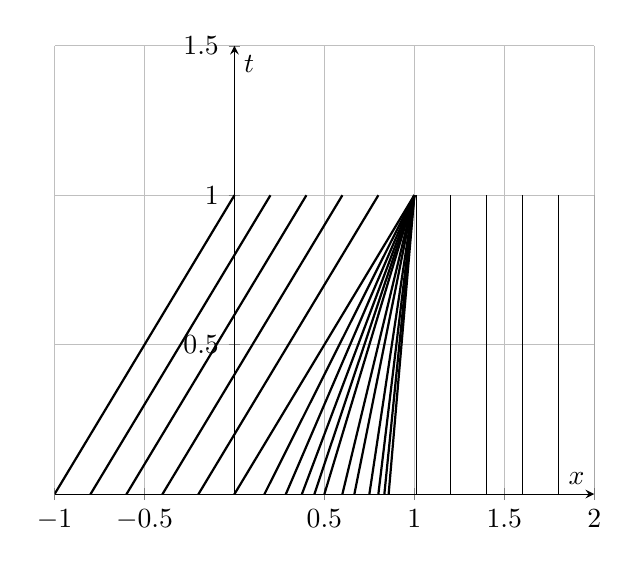
\begin{tikzpicture}
        \begin{axis}[
                xlabel={$x$}, ylabel={$t$},
                xmin=-1, xmax=2, ymin=0, ymax=1.5,
                axis lines=middle, grid=major,
                samples=20, domain=-2:1, legend pos=outer north east
            ]

            % Plot characteristics for u_0(x) = 1 for x <= 0

            \addplot[black, thick, domain=-2:-0.6] {x -0.4}; % Characteristic with slope 1
            \addplot[black, thick, domain=-2:-0.8] {x - 0.2}; % Characteristic with slope 1
            \addplot[black, thick, domain=-1:1] {x}; % Characteristic with slope 1
            \addplot[black, thick, domain=-1:0.8] {x + 0.2}; % Characteristic with slope 1
            \addplot[black, thick, domain=-1:0.6] {x + 0.4}; % Characteristic with slope 1
            \addplot[black, thick, domain=-1:0.4] {x + 0.6}; % Characteristic with slope 1
            \addplot[black, thick, domain=-1:0.2] {x + 0.8}; % Characteristic with slope 1
            \addplot[black, thick, domain=-1:0] {x + 1}; % Characteristic with slope 1

            % Plot characteristics for u_0(x) = 2 - 2x for 0 < x < 1
            \addplot[black, thick,domain=0:1] {x - (2 - 2*x) * 0.1};
            \addplot[black, thick,domain=0:1] {x - (2 - 2*x) * 0.2};
            \addplot[black, thick,domain=0:1] {x - (2 - 2*x) * 0.3};
            \addplot[black, thick,domain=0:1] {x - (2 - 2*x) * 0.4};
            \addplot[black, thick,domain=0:1] {x - (2 - 2*x) * 0.5};
            \addplot[black, thick,domain=0:1] {x - (2 - 2*x) * 0.75};
            \addplot[black, thick,domain=0:1] {x - (2 - 2*x)};
            \addplot[black, thick,domain=0:1] {x - (2 - 2*x) * 1.5};
            \addplot[black, thick,domain=0:1] {x - (2 - 2*x) * 2};
            \addplot[black, thick,domain=0:1] {x - (2 - 2*x) * 2.5};
            \addplot[black, thick,domain=0:1] {x - (2 - 2*x) *3};

            % Plot characteristics for u_0(x) = 0 for x > 1
            \draw[color=black]
            (axis cs:1.01, 0) -- (axis cs:1.01, 1);
            \draw[color=black]
            (axis cs:1.2, 0) -- (axis cs:1.2, 1);
            \draw[color=black]
            (axis cs:1.4, 0) -- (axis cs:1.4, 1);
            \draw[color=black]
            (axis cs:1.6, 0) -- (axis cs:1.6, 1);
            \draw[color=black]
            (axis cs:1.8, 0) -- (axis cs:1.8, 1);
            \draw[color=black]
            (axis cs:2, 0) -- (axis cs:2, 1);
        \end{axis}
    \end{tikzpicture}
\end{center}
that the characteristic do not intersect at least until \(t=1\).
Therefore, the function \(u(x,t)\) is defined continuous in \(\real \times [0, 1)\) and it is written as
\[
    u(x,t) = \begin{cases}
        1,                 & x \leq t,  \\
        \frac{2-2x}{1-2t}, & t < x < 1, \\
        0,                 & x \geq 1.
    \end{cases}
\]
We want to extend the solution to \(t > 1\). We need the solution to undergo a
jump, so given \(x = \eta(t)\) the curve of discontinuity, we have that
\[
    u(x, t) = \begin{cases}
        u_- = 1, & x < \eta(t) \\
        u_+ = 0, & x > \eta(t)
    \end{cases}
\]
The jump conditions states that
\[
    \eta'(t) \cdot \left[u_+ - u_-\right] = \left[B(u_+) - B(u_-)\right] \quad \text{on } \Gamma
\]
Here we have that \(B(u) = \frac{u^2}{2}\), so the jump condition becomes
\[
    \eta'(t) = \frac{u_+^2 - u_-^2}{u_+ - u_-} = \frac{1}{2}
\]
and the solution is
\[
    \eta(t) = \frac{t}{2} + C
\]
But, we know that \(\eta(1) = 1\), so \(C = 1/2\) and the solution is
\[
    u(x,t) = \begin{cases}
        1, & x < \frac{1}{2}(t+1), \\
        0, & x > \frac{1}{2}(t+1).
    \end{cases}
\]
Which is a discontinuous solution.

To satisfy the entropy condition we need to have that the characteristics on
both sides of the shock point towards the shock. To ensure this the condition
\(s = \eta'(t)\) should be less than the speed of the characteristic on the
right side and greater than the speed of the characteristic on the left side.
We have
\begin{align*}
    \text{Left side:}  & \quad u_-(x,t) = 1, \Rightarrow \frac{1}{2} < 1, \quad \text{True} \\
    \text{Right side:} & \quad u_+(x,t) = 0, \Rightarrow \frac{1}{2} > 0, \quad \text{True}
\end{align*}
Therefore the solution satisfies the entropy condition.

\newpage
\begin{exercise}
    Let \(\Omega \subset \real^n\) \(n \geq 2\) be a bounded open domain with \(\partial\Omega \in C^\infty\) and consider the boundary value problem
    \[
        \begin{cases}
            -\Delta u = f & \Omega         \\
            u = 0         & \partial\Omega
        \end{cases}
        \tag*{(P)}
    \]
    \begin{enumerate}
        \item Assuming that \(f \in H^{-1}(\Omega)\), write the weak formulation of (P).
        \item Prove that this problem admits a unique weak solution.
        \item Show that the unique solution \(u\) satisfies the Dirichlet principle.
        \item If \(f \in L^2(\Omega)\), in which space dimension \(n\) is it guaranteed that
              the solution \(u\) belongs to \(C^0(\overline{\Omega})\)?
    \end{enumerate}
\end{exercise}
\begin{enumerate}
    \item We start by writing the weak formulation of the problem. First we define a
          suitable function space, in this case we have \(V \in H^1_0(\Omega)\). We
          multiply the equation by a test function \(v \in V\) and obtain
          \[
              \begin{split}
                  -\int_\Omega \Delta u v \, dx = \int_\Omega f v \, dx \qquad \forall v \in V
              \end{split}
          \]
          We integrate by parts the left-hand side and obtain
          \[
              \begin{split}
                  \int_\Omega \grad u \grad v \, dx = \underbrace{\langle f, v \rangle}_{\text{bc } f \in H^{-1}} \qquad \forall v \in V
              \end{split}
          \]
          Then we obtain the weak formulation of the problem
          \[
              \begin{split}
                  \text{Find } u \in H^1_0(\Omega) \text{ such that } \int_\Omega \grad u \grad v \, dx =  \langle f, v \rangle \qquad \forall v \in V
              \end{split}
          \]
    \item Then we state the Dirichlet principle for the homogeneous Dirichlet problem
          \begin{remark}
              Let \(\Omega \subset \real^n\) be a bounded and Lipschitz domain and let \(f \in H^{-1}(\Omega), \alpha \geq 0\). Then the problem (P) admits a unique solution \(u \in V\) such that
              \[
                  \int_\Omega \grad u \grad v \, dx = \langle f, v \rangle \qquad \forall v \in V
              \]
              Moreover, \(u\) is the unique minimizer of the functional
              \[
                  J(u) = \frac{1}{2} \int_\Omega \abs{\grad u}^2 \, dx - \langle f, u \rangle
              \]
          \end{remark}
          A sketch of the proof goes as follows. We start by defining the functional
          \begin{align*}
              a: V \times V & \longrightarrow \real                         \\
              (u, v)        & \longmapsto \int_\Omega \grad u \grad v \, dx
          \end{align*}
          We have that \(a(u,v)\) is a continuous and coercive bilinear form. Then we can apply the Lax-Milgram theorem to obtain the existence of a unique solution \(u \in V\).

          To prove that the solution is the unique minimizer of the functional we need to
          observe that the functional \(J(u)\) is convex.
    \item Now we will prove that the unique solution \(u\) is the minimizer of the
          functional \(J(u)\). We start by recalling \(J(u)\)
          \[
              J(u) = \frac{1}{2} \int_\Omega \abs{\grad u}^2 \, dx - \langle f, u \rangle
          \]
          Assume \(\bar{u} \in V\) is a solution of the weak formulation of the problem.
          Then \(\exists w \in V\) such that \(u = \bar{u} + w\). We have that
          \[
              \begin{split}
                  J(u) = J(\bar{u} + w) = \frac{1}{2} \int_\Omega \abs{\grad \bar{u} + \grad w}^2 \, dx - \langle f, \bar{u} + w \rangle = \\
                  =J(\bar{u}) + \underbrace{\frac{1}{2}\int_\Omega \abs{\grad w}^2 \, dx}_{\geq 0} + \underbrace{\int_\Omega \grad \bar{u} \grad w \, dx - \langle f, w \rangle}_{\text{\tiny def. of weak solution } = 0} \geq J(\bar{u})
              \end{split}
          \]
          So, if \(w \neq 0\) we have that \(J(u) > J(\bar{u})\). Then, if \(\bar{u}\) is
          the weak solution, it is also the minimizer of the functional.
    \item To prove that the solution \(u\) belongs to \(C^0(\overline{\Omega})\) we need
          Sobolev embedding. We know that \(f \in H^m(\Omega)\) implies that \(u \in
          H^{m+2}(\Omega)\). We have that \(f \in L^2 \Rightarrow u \in H^2\) By Sobolev
          embedding, \(u \in C^0(\overline{\Omega})\) if \(n < 2s\), where \(s\) is the
          Sobolev exponent. Therefore, if \(n < 4\) we have that the solution \(u\)
          belongs to \(C^0(\overline{\Omega})\).
\end{enumerate}

\newpage
\subsection{January 2024}
\begin{exercise}
    For given constants \(\alpha, \beta, \gamma \in \real\), consider the Cauchy problem
    \[
        \begin{cases}
            u_{t} - \alpha u_{xx} - \beta u_{x}^4 + \gamma u^3u_x = 0, & (x,t) \in \real \times (0, \infty), \\
            u(x,0) = u_0(x),                                           & x \in \real,                        \\
        \end{cases}
        \tag*{(P)}
    \]
    \begin{enumerate}
        \item Find conditions on \(\alpha, \beta, \gamma\) ensuring mass conservation for
              regular solutions of (P).
        \item Find conditions on \(\alpha, \beta, \gamma\) ensuring momentum conservation for
              regular solutions of (P).
        \item When \(\beta = 0\), find a first-order ODE on \(g\) giving a necessary
              condition to have solitary wave solutions of (P).
    \end{enumerate}
\end{exercise}
\begin{enumerate}
    \item To have mass conservation we need \(\frac{\partial}{\partial t}\int_\real
          u(x,t) \, dx = 0\). We have that
          \[
              \begin{split}
                  \frac{\partial}{\partial t}\int_\real u(x,t) \, dx = \int_\real u_t(x,t) \, dx = \int_\real \left(- \alpha u_{xx} - \beta u_{x}^4 - \gamma u^3u_x\right) \, dx =
              \end{split}
          \]
          Let's see each term separately
          \[
              \begin{split}
                  \int_\real - \alpha u_{xx} \, dx = -\alpha \left.u_x\right|_\real = 0
              \end{split}
          \]
          This term goes to zero because we have that \(u \in \mathcal{S}(\real)\), so it
          is zero \(\forall \alpha\). The third term becomes
          \[
              \begin{split}
                  \int_\real - \gamma u^3u_x \, dx = -\frac{\gamma}{4} \left. u^4 \right|_\real = 0
              \end{split}
          \]
          same as before, this term goes to zero because we have that \(u \in
          \mathcal{S}(\real)\), so it is zero \(\forall \gamma\). The second term becomes
          \[
              \begin{split}
                  \int_\real - \beta u_{x}^4 \, dx = 0 \iff \beta = 0
              \end{split}
          \]
          Therefore, the condition for mass conservation is \(\beta = 0\).
    \item To have momentum conservation we need \(\frac{\partial}{\partial t}\int_\real
          u(x,t)^2 \, dx = 0\). We have that
          \[
              \begin{split}
                  \frac{\partial}{\partial t}\int_\real u(x,t)^2 \, dx = \int_\real 2u(x,t)u_t(x,t) \, dx = \int_\real 2u(x,t)\left(- \alpha u_{xx} - \beta u_{x}^4 - \gamma u^3u_x\right) \, dx
              \end{split}
          \]
          Let's see each term separately
          \[
              \begin{split}
                  -2\alpha \int_\real u u_{xx} \, dx = -\alpha \int_\real (u_x)^2 \, dx = 0 \iff \alpha = 0
              \end{split}
          \]
          The second term becomes
          \[
              \begin{split}
                  -2\beta \int_\real u u_{x}^4 \, dx = 0 \iff \beta = 0
              \end{split}
          \]
          The third term becomes
          \[
              \begin{split}
                  -2\gamma \int_\real u^4u_x \, dx = -\frac{\gamma}{5} \int_\real (u^5)_x \, dx = 0
              \end{split}
          \]
          Therefore, the condition for momentum conservation is \(\alpha = \beta = 0\).
    \item When \(\beta = 0\) we have that the equation becomes
          \[
              \begin{split}
                  u_{t} - \alpha u_{xx} + \gamma u^3u_x = 0
              \end{split}
          \]
          Solitary waves are solutions of the form \(u(x,t) = g(x + ct)\). We substitute
          this into the equation and obtain
          \[
              \begin{split}
                  cg'(x + ct) - \alpha g''(x + ct) + \gamma g(x + ct)^3g'(x + ct) = 0
              \end{split}
          \]
          We perform the change of variables \(s = x + ct\) and obtain
          \[
              \begin{split}
                  cg'(s) - \alpha g''(s) + \gamma g(s)^3g'(s) = 0
              \end{split}
          \]
          We can rewrite this as
          \[
              \begin{split}
                  \frac{d}{ds} \left[ cg(s) - \alpha g'(s) + \frac{\gamma}{4} g(s)^4 \right] = 0
              \end{split}
          \]
          Integrating this equation we obtain
          \[
              \begin{split}
                  cg(s) - \alpha g'(s) + \frac{\gamma}{4} g(s)^4 = C
              \end{split}
          \]
          where \(C\) is a constant. This is the first-order ODE that gives a necessary
          condition to have solitary wave solutions of the problem.
\end{enumerate}

\newpage
\begin{exercise}
    Let \(\Omega \subset \real^n (n \geq 2)\) be a bounded smooth domain, let \(a\) be a measurable function in \(\Omega\).
    Consider the problem
    \[
        \begin{cases}
            - \Delta u = a(x) u^3 & \Omega         \\
            u = 0                 & \partial\Omega
        \end{cases}
        \tag*{(P)}
    \]
    Under which assumptions on the space dimension n can we write a variational
    formulation of problem (P) in \(H^1_0(\Omega)\)?

    For each of these dimensions find the most general assumptions on \(a\) that
    allow to write the variational formulation.

    Finally, write the variational formulation.
\end{exercise}

First, a quick reminder on Sobolev embedding, which will be very useful a.e. in
this document
\begin{remark}
    Let \(\Omega \subseteq \real^n\) open with \(\partial\Omega \in \text{Lip}\), \(s \geq 0\),
    \[
        H^s(\Omega) \subset
        \begin{cases}
            L^p(\Omega) \qquad \forall \, 2 \leq p \leq 2^* & \text{if } n > 2s \\
            L^p(\Omega) \qquad \forall \, 2 \leq p < \infty & \text{if } n = 2s \\
            C^0(\bar{\Omega})                               & \text{if } n < 2s
        \end{cases}
    \]
    Increasing \(s\) increases the regularity, while increasing \(n\) decreases it.

    The exponent \(2^*\) is called critical exponent and is defined as \(2^*
    \coloneqq \frac{2n}{n - 2s}\).

    If \(\Omega\) is bounded, all these embeddings are compact except \(H^s(\Omega)
    \subset L^{2^*}\) when \(n > s\).
\end{remark}

Since we want to know the variational formulation in \(H^1_0\) we have \(s =
1\) and need to check \(n = 2, n \geq 3\). Remember a variational formulation
makes sense if \(\int_\Omega fv < \infty\).
\begin{itemize}
    \item[\(n = 2\).] In this case we have \(u, v \in H^1_0(\Omega)\), so by Sobolev embedding we know \(u, v \in L^p(\Omega)\) for \(2 \leq p < \infty\).
          \[
              \abs{\int_\Omega a(x) u^3 v}  \, dx \leq \int_\Omega \abs{a(x)} \abs{u^3} \abs{v} \, dx \underset{Holder}{\leq} \left(\int_\Omega \abs{a(x)}^r\right)^{\frac{1}{r}} \left(\int_\Omega \abs{u^3}^p \right)^{\frac{1}{p}} \left(\int_\Omega \abs{v}^q \right)^{\frac{1}{q}} < \infty.
          \]
          To use Holder inequality we need to find \(r, p, q\) such that \(\frac{1}{r} +
          \frac{1}{p} + \frac{1}{q} = 1\). We see that,
          \[
              \frac{1}{r} + \frac{1}{p} + \frac{1}{q} = 1 \iff a(x) \in L^r(\Omega) \qquad \text{with } r > 1
          \]
    \item[\(n \geq 3\).] In this case we have \(u, v \in H^1_0(\Omega)\), so by Sobolev embedding we know \(u, v \in L^p(\Omega)\) for \(2 \leq p \leq 2^*\).
          We proceed as before, using Holder inequality, but decide to use \(p = \frac{2^*}{3}\) and \(q = \frac{1}{2^*}.\)
          \[
              \abs{\int_\Omega a(x) u^3 v}  \, dx \leq \int_\Omega \abs{a(x)} \abs{u^3} \abs{v} \, dx \underset{\mathclap{Holder}}{\leq} \left(\int_\Omega \abs{a(x)}^r\right)^{\frac{1}{r}} \left(\int_\Omega \abs{u}^{2^*} \right)^{\frac{3}{2^*}} \left(\int_\Omega \abs{v}^{2^*} \right)^{\frac{1}{2^*}} < \infty.
          \]
          In this case Holder inequality gives us
          \[
              \frac{1}{r} + \frac{3}{2^*} + \frac{1}{2^*} = 1 \iff \frac{1}{r} = 1 - \frac{4}{2^*} \iff r = \frac{2^*}{2^* - 4}
          \]
          Substituting \(2^* = \frac{2n}{n - 2}\) we get \(r = \frac{n}{-n + 4}\). Since
          \(r > 0\) we need \(n < 4\). In this case we have \(a(x) \in L^3(\Omega)\) for
          \(n = 3\), but also \(a(x) \in L^\infty(\Omega)\) for \(n = 4\).
\end{itemize}

At this point we can write the weak formulation of the problem. We multiply the
equation by a test function \(v \in H^1_0(\Omega)\) and obtain
\[
    \int_\Omega - \Delta u v \, dx = \int_\Omega a(x) u^3 v \, dx \qquad \forall v \in H^1_0(\Omega)
\]
We integrate by parts the left-hand side and obtain
\[
    \int_\Omega \nabla u \nabla v \, dx = \int_\Omega a(x) u^3 v \, dx \qquad \forall v \in H^1_0(\Omega)
\]
This is the weak formulation of the problem. This is well posed if
\begin{table}[h]
    \centering
    \begin{tabular}{|c|c|}
        \hline
        Dimension  & Assumptions on $a(x)$        \\
        \hline
        $n = 2$    & $a \in L^r(\Omega)$, $r > 1$ \\
        $n = 3$    & $a \in L^3(\Omega)$          \\
        $n = 4$    & $a \in L^\infty(\Omega)$     \\
        $n \geq 5$ & No variational formulation   \\
        \hline
    \end{tabular}
\end{table}

\newpage
\begin{exercise}
    Let \(\Omega \subset \real^2\) be a bounded, simply connected, smooth domain and \(\eta > 0\). Consider the inhomogeneous Dirichlet boundary value problem for the unforced Navier-Stokes equations
    \[
        \begin{cases}
            -\eta \Delta u + (u \cdot \grad )u + \grad p = f & \Omega         \\
            \div u = 0                                       & \Omega         \\
            u = (1,1)                                        & \partial\Omega
        \end{cases}
        \tag*{(P)}
    \]
    \begin{enumerate}
        \item Find an explicit solenoidal extension of the boundary datum.
        \item Prove that (P) admits a unique solution \(u\) for any \(\eta > 0\).
    \end{enumerate}
\end{exercise}

\begin{enumerate}
    \item We start by finding an explicit solenoidal extension of the boundary datum. We
          have that the boundary datum is \(u = (1,1)\) on \(\partial\Omega\). We can
          extend this to the whole domain by defining
          \[
              \begin{split}
                  u(x) = (1,1) \qquad \forall x \in \Omega
              \end{split}
          \]
          This is a solenoidal extension of the boundary datum because \(\div u = 0\).
    \item We will now prove uniqueness thanks to the theorem
          \begin{remark}[Uniqueness stationary N-S]
              If \(\exists \gamma > 0\) such that \(\norm{f}_{\bm{V'}} < \gamma\), then the problem (P) admits a unique solution.
          \end{remark}
          For the proof we start with the weak formulation of the problem.
          \[
              \begin{split}
                  \eta \int_\Omega \grad u : \grad v \, dx + \int_\Omega (u \cdot \grad) u \cdot v \, dx = \langle f, v \rangle \qquad \forall v \in \bm{V}
              \end{split}
          \]
          and define trilinear form
          \[
              \begin{split}
                  b(u, v, w) = \int_\Omega (u \cdot \grad) v \cdot w \, dx
              \end{split}
          \]
          Now we take \(v = u\) and obtain the following a priori bound
          \[
              \begin{split}
                  \eta \norm{u}_{\bm{V}}^2 = \langle f, u \rangle - \underbrace{\cancel{b(u, u, u)}}_{=0} \leq \norm{f}_{\bm{V'}} \norm{u}_{\bm{V}}
              \end{split}
          \]
          Thanks to the Cauchy-Schwarz inequality. We have that
          \[
              \begin{split}
                  \norm{u}_{\bm{V}} \leq \frac{\norm{f}_{\bm{V'}}}{\eta}
              \end{split}
          \]
          Now assume the existence of two solutions \(u_1\) and \(u_2\):
          \begin{align*}
              \eta \int_\Omega \grad u_1 : \grad v \, dx + b(u_1, u_1, v) & = \langle f, v \rangle \qquad \forall v \in \bm{V} \\
              \eta \int_\Omega \grad u_2 : \grad v \, dx + b(u_2, u_2, v) & = \langle f, v \rangle \qquad \forall v \in \bm{V}
          \end{align*}
          Subtracting the two equations with \(w = u_1 - u_2\) we obtain
          \[
              \begin{split}
                  \eta \int_\Omega \grad w : \grad w \, dx + b(u_1, u_1, v) - b(u_2, u_2, v) = 0 \qquad \forall v \in \bm{V}
              \end{split}
          \]
          We see that
          \begin{align*}
              b(u_1, u_1, v) - b(u_2, u_2, v) & = b(u_1, u_1, v) - b(u_1, u_2, v) + b(u_1, u_2, v) - b(u_2, u_2, v) \\
                                              & = b(u_1, u_1 - u_2, v) + b(u_1 - u_2, u_2, v)                       \\
                                              & = b(u_1, w, v) + b(w, u_2, v)                                       \\
          \end{align*}
          We can now rewrite the equation as
          \[
              \begin{split}
                  \eta \int_\Omega \grad w : \grad v \, dx= -b(w, u_2, v) - b(u_1, w, v) \qquad \forall v \in \bm{V}
              \end{split}
          \]
          Choosing \(v = w\) we obtain \(\eta \norm{w}_{\bm{V}}^2 = -b(w, u_2, w) -
          \cancel{b(u_1, w, w)}\). We have that
          \[
              \begin{split}
                  \eta \norm{w}_{\bm{V}}^2 = -b(w, u_2, w) \leq C \norm{w}_{\bm{V}}^2 \norm{u_2}_{\bm{V}}
              \end{split}
          \]
          where \(C\) is a constant depending on the domain. Substituting the a priori
          bound we have that
          \[
              \begin{split}
                  \eta \norm{w}_{\bm{V}}^2 \leq C_\Omega \frac{\norm{f}_{\bm{V'}}}{\eta} \norm{w}_{\bm{V}}^2
              \end{split}
          \]
          We can see that if
          \[
              \begin{split}
                  C_\Omega \frac{\norm{f}_{\bm{V'}}}{\eta} < \eta \Rightarrow \norm{w}_{\bm{V}} = 0 \Rightarrow w = 0 \Rightarrow \gamma = \frac{\eta^2}{C_\Omega}
              \end{split}
          \]
          we have that the problem admits a unique solution.
\end{enumerate}

\newpage
\begin{exercise}
    Prove that there exists at most one smooth solution \(u\) for the beam equation
    \[
        \begin{cases}
            u_{tt} + u_{xxxx} = f                         & (x,t) \in (0,1) \times (0, T) \\
            u(0, t) = u(1, t) = u_x(0, t) = u_x(1, t) = 0 & t \in [0, T]                  \\
            u(x, 0) = g(x), u_t(x, 0) = h(x)              & x \in [0, 1]
        \end{cases}
        \tag*{(P)}
    \]
    where \(f \in C^1([0,1] \times [0, T])\), \(g, h \in C^1([0,1])\) are given
    functions.
\end{exercise}

We start by assuming that there are two solutions \(u_1\) and \(u_2\). We
define \(w = u_1 - u_2\). We have that \(w\) satisfies the homogeneous beam
equation
\[
    \begin{cases}
        w_{tt} + w_{xxxx} = 0                         & (x,t) \in (0,1) \times (0, T) \\
        w(0, t) = w(1, t) = w_x(0, t) = w_x(1, t) = 0 & t \in [0, T]                  \\
        w(x, 0) = 0, w_t(x, 0) = 0                    & x \in [0, 1]
    \end{cases}
\]
We multiply the equation by \(w_t\) and integrate over \(x\)
\[
    \begin{split}
        \int_0^1 w_t w_{tt} + w_t w_{xxxx} \, dx = 0
    \end{split}
\]
The first term becomes
\[
    \begin{split}
        \int_0^1 w_t w_{tt} \, dx = \frac{1}{2} \frac{\partial}{\partial t} \int_0^1 w_t^2 \, dx = \frac{1}{2} \frac{\partial}{\partial t} \norm{w_t}_{L^2}^2
    \end{split}
\]
The second term becomes
\[
    \begin{split}
        \int_0^1 w_t w_{xxxx} \, dx = \cancel{\left. w_t w_{xxx} \right|_0^1} - \int_0^1 w_{tx} w_{xxx} \, dx = - \int_0^1 w_{tx} w_{xxx} \, dx = \\
        = -\cancel{\left. w_{tx} w_{xx} \right|_0^1} + \int_0^1 w_{txx} w_{xx} \, dx = \int_0^1 w_{txx} w_{xx} \, dx
    \end{split}
\]
which can be rewritten as
\[
    \begin{split}
        \int_0^1 w_{txx} w_{xx} \, dx = \frac{1}{2} \frac{\partial}{\partial t} \int_0^1 w_{xx}^2 \, dx = \frac{1}{2} \frac{\partial}{\partial t} \norm{w_{xx}}_{L^2}^2
    \end{split}
\]
Therefore we have that
\[
    \begin{split}
        \frac{1}{2} \frac{\partial}{\partial t} \left(\norm{w_t}_{L^2}^2 + \norm{w_{xx}}_{L^2}^2\right) = 0
    \end{split}
\]
which implies that
\[
    \begin{split}
        \norm{w_t}_{L^2}^2 + \norm{w_{xx}}_{L^2}^2 = \text{ constant} = F(t)
    \end{split}
\]
We have that \(F(t) = \text{ const.}\) and
\[
    \begin{split}
        F(0) = \norm{w_t(x, 0)}_{L^2}^2 + \norm{w_{xx}(x, 0)}_{L^2}^2 = 0
    \end{split}
\]
Since \(w_t(x, 0) = 0\) and \(w(x,0) = 0 \Rightarrow w_{xx}(x, 0) = 0\).
Therefore \(F(0) = 0\). We have that \(F(t) = 0\) for all \(t \in [0, T]\).
This implies that \(w_t = 0\) and \(w_{xx} = 0\). Therefore \(w = 0\) and the
solution is unique.

\newpage
\subsection{February 2024}
\begin{exercise}
    Let \(\Omega \subset \real^2\) be a bounded open set of class \(C^1\), and let \(f \in L^2(\Omega)\). Consider the Dirichlet problem
    \begin{equation*}
        \begin{cases}
            u_{t} - \left(\partial_x^2 u +  \partial_y^2 u - 2 \partial_{xy} u\right) = f, & \text{in } \Omega \times (0, T),          \\
            u = 0,                                                                         & \text{on } \partial \Omega \times (0, T), \\
            u(x,0) = u_0(x),                                                               & x \in \Omega,                             \\
        \end{cases}
        \tag{(P)}
    \end{equation*}
    \begin{enumerate}
        \item For a suitable symmetric matrix \(A\), write the PDE appearing in (P) in the
              form \(u_{tt} - \div(A \grad u) = f\).
        \item Write the weak formulation of (P).
        \item Sketch the proof of existence and uniqueness of a solution of (P), explaining
              to which functional spaces is expected to belong.
    \end{enumerate}
\end{exercise}
\begin{enumerate}
    \item We start by writing the PDE in the form \(u_{tt} - \div(A \grad u) = f\). We
          have that
          \[
              u_{t} - \left(A_{11} u_{xx} + A_{22} u_{yy} + 2A_{12} u_{xy}\right) = f.
          \]
          We can write the matrix \(A\) as
          \[
              A = \begin{pmatrix}
                  2 & 1 \\
                  1 & 1
              \end{pmatrix}
          \]
          and the PDE becomes
          \[
              u_{t} - \div (A \grad u) = f.
          \]
    \item To write the weak formulation we choose an adequate Hilbert triplet, keeping in
          mind that this problem is equipped with Dirichlet boundary conditions. We can
          choose the Hilbert triplet
          \[
              V = H^1_0(\Omega) \subset H = L^2(\Omega) \subset V' = H^{-1}(\Omega).
          \]
          The weak formulation of the problem is then obtained by multiplying the
          equation by a test function \(v \in V\) and integrating over \(\Omega\)
          \begin{align*}
              \int_\Omega f(t) v \, dx & = \int_\Omega u_{t} v \, dx + \int_\Omega \div(A \grad u)v \, dx =                                                                                  \\
                                       & = \int_\Omega u_{t} v \, dx - \cancel{\int_{\partial\Omega} \partial_\nu u v \, d\sigma} + \int_\Omega \left[A \grad u \cdot \grad v\right] \, dx = \\
                                       & = \int_\Omega u_{t} v \, dx + \int_\Omega \underbrace{A \grad u \cdot \grad v}_{B(u, v)} \, dx
          \end{align*}
          The weak formulation of the problem is then
          \[
              \begin{split}
                  \text{Find } u(t) \in L^2([0, T]; V)\cap C^0([0, T]; H)\text{ such that } \\
                  u' \in L^2([0, T];H)\text{ and }                                          \\
                  \begin{cases}
                      \langle u_{t}(t), v \rangle + B(u(t), v) = (f(t), v)_H \\
                      u(0) = u_0,
                  \end{cases}\quad \forall v \in V, \text{ in } \mathcal{D}(0, T).
              \end{split}
          \]
    \item To sketch the proof of existence and uniqueness of a solution of the problem we
          need to use the Galerkin method. The advantage of the Galerkin method is that
          is finite-dimensional, so we can have as much regularity as we want. Let
          \(\left\{V_m\right\}\) be a Galerkin sequence for \(V\), with a basis
          \(\left\{w_m \right\}\). We can now write the weak formulation of the problem
          in the Galerkin space
          \[
              \begin{split}
                  \text{Find } u_m \in H^1((0, T); V_m) \text{ such that } \\
                  \begin{cases}
                      \left(u_m'(t), v_m\right)_H + B(u_m(t), v_m) = \langle f(t), v_m \rangle_H  \quad \forall v_m \in V_m \\
                      u_m(0) = P_m u_0
                  \end{cases}
              \end{split}
          \]
          We now have a finite number of linear ODEs, and for \(1 \leq k \leq m\) we have
          \[
              u_m(t) = \sum_{k=1}^m g_k^m(t) w_k^m
          \]
          So we want to solve the following system
          \[
              \begin{cases}
                  g_m'(t) + B_m g_m(t) = \gamma_m(t) \\
                  g_m(0) = g_0^m,
              \end{cases}
          \]
          Since \(g_m(t)\) is the unique solution of the system, we have that \(g_m(t)\)
          uniquely determines \(u_m(t)\). Then it is possible, taking \(v_m = u_m\) to
          obtain
          \[
              \frac{1}{2}\frac{d}{dt}\norm{u_m(t)}_H^2 + B(u_m(t), u_m(t)) = \langle f(t), u_m(t) \rangle \quad \forall t \in (0, T)
              \tag*{(E)}
          \]
          Integrating and using some inequalities gives us two a priori bounds
          \[
              \norm{u_m(t)}_{L^\infty(0, T; H)} \leq K_1 \quad \text{and} \quad \norm{u_m(t)}_{L^2(0, T; V)} \leq K_2
          \]
          Since the bounds are in \(L^2(0, T; V)\) and \(L^\infty(0, T; H)\), we have
          that up to a subsequence
          \begin{align*}
              \int_0^T \left(u_m(t), v(t)\right)_H \, dt & \to \int_0^T \left(u(t), v(t)\right)_H \, dt \quad \forall v \in L^1(0, T; H) \\
              \int_0^T \left(u_m(t), v(t)\right)_V \, dt & \to \int_0^T \left(u(t), v(t)\right)_V \, dt \quad \forall v \in L^2(0, T; V)
          \end{align*}
          With these converges we are able to manage \(B(u_m, v_m)\) and \(\langle f, v_m \rangle\). We need some bounds on \(\langle u_t, v \rangle\). Using the weak derivative definition we can ``free'' the time derivative and obtain
          \[
              \begin{split}
                  - \int_0^T \left(u_m(t), v_t(t)\right)_H \phi'(t) \, dt - \left(u_m(0), v(0)\right)_H \phi(0) \\\to -\int_0^T \left(u(t), v_t(t)\right)_H \phi'(t) \, dt - \left(u(0), v(0)\right)_H \phi(0)
              \end{split}
          \]
          We can integrate by parts and obtain
          \[
              \begin{split}
                  -\int_0^T \left(u(t), v\right)_H \phi'(t) \, dt + \left(u(0), v(0)\right)_H \phi(0) = \int_0^T \langle u_t(t), v \rangle \phi(t) \, dt
              \end{split}
          \]
          We have then that
          \[
              \begin{split}
                  \langle u_t(t), v \rangle = - B(u(t), v) + \langle f(t), v \rangle
              \end{split}
          \]
          Since \(B(u,v)\) is a bilinear continuous and coercive form, if we fix \(v\) we
          have that \(B(u, v)\) is a linear continuous functional. Then we have
          \[
              \begin{split}
                  \langle u_t(t), v \rangle = \langle \mathcal{L}(t), v \rangle
              \end{split}
          \]
          with \(\mathcal{L}(t) = -B(u(t), v) + \langle f(t), v \rangle \in L^2(0, T;
          V')\). Then
          \[
              \begin{cases}
                  u \in L^2(0, T; V)   \\
                  u' \in L^2(0, T; V') \\
              \end{cases}
              \Rightarrow u \in C^0([0, T]; H).
          \]
          Then we take two solutions \(u_1\) and \(u_2\) and we have that \(w = u_1 -
          u_2\) . Putting \(w\) in (E) we obtain
          \[
              \begin{cases}
                  \frac{1}{2} \frac{d}{dt} \norm{w(t)}_H^2 + B(w(t), w(t)) = 0 \\
                  w(0) = 0
              \end{cases}
          \]
          Since both \(\norm{w(t)}_H^2\) and \(B(w(t), w(t))\) are positive, we have that
          \(\frac{1}{2} \frac{d}{dt} \norm{w(t)}_H^2 \leq 0\). This implies that \(w =
          0\) and the solution is unique.
\end{enumerate}

\newpage
\begin{exercise}
    Consider the conservation law with two different initial conditions
    \begin{equation*}
        a)\,\begin{cases}
            u_t - u^3 u_x = 0,    & x \in \real, t > 0, \\
            u(x,0) = \sqrt[3]{x}, & x \in \real,
        \end{cases}
        \qquad
        b)\,\begin{cases}
            u_t - u^3 u_x = 0,    & x \in \real, t > 0, \\
            u(x,0) = -\sqrt[3]{x} & x \in \real.
        \end{cases}
    \end{equation*}
    Determine the maximal domain \(A\) of definition of the solution as continuous function: explain if they are also of class \(C^1(A)\) and satisfy the entropy condition.
\end{exercise}
\begin{enumerate}
    \item[\textbf{a)}] We look for solutions \(u(x, t) \in C^1(\real \times (0, \infty))\) that satisfy the conservation law and the initial condition.
          Its characteristics are given by
          \[
              \frac{du}{dt} = \frac{dt}{ds} \frac{du}{dt} + \frac{dx}{ds} \frac{du}{dx} = 0
          \]
          means that \(u\) is constant along the characteristics and then
          \[
              u(x,t) = u(x_0,0) = \sqrt[3]{x_0}
          \]
          with \(t=s\) since the initial condition is given at \(t=0\).
          \[
              \frac{dx}{ds} = u_0^3 \quad \Rightarrow \quad x(s) = x_0 + s u_0^3
          \]
          Since \(u_0^3 = (\sqrt[3]{x_0})^3 = x_0\), we have that \(x(s) = x_0 + s x_0 =
          x_0(1+s)\). We can then write the solution as
          \[
              x(s) = x_0 + s x_0 = x_0(1+s) \quad \Rightarrow \quad x_0 = \frac{x}{1+s}.
          \]
          The solution is then
          \[
              u(x,t) = \sqrt[3]{\frac{x}{1+t}}.
          \]
          This is a classical solution that remains smooth for all \(x \in \real\) and
          \(t > 0\), so the maximal domain of definition is \(A = \real \times (0,
          \infty)\). Let's compute the derivatives of \(u\)
          \begin{align*}
              u_x(x,t) & = \frac{1}{3} \frac{1}{\sqrt[2]{\frac{x}{1+t}}^2}         \\
              u_t(x,t) & = -\frac{1}{3(1+t)^2} \frac{1}{\sqrt[3]{\frac{x}{1+t}}^2}
          \end{align*}
          These are not continuous at \(x=0\), so the solution is not of class \(C^1(A)\). Since we do not have a discontinuity in our solution, the entropy condition is satisfied.
    \item[\textbf{b)}] Now we look at the second case.

          Its characteristics are given by
          \[
              \frac{du}{dt} = \frac{dt}{ds} \frac{du}{dt} + \frac{dx}{ds} \frac{du}{dx} = 0
          \]
          means that \(u\) is constant along the characteristics and then
          \[
              u(x,t) = u(x_0,0) = -\sqrt[3]{x_0}
          \]
          with \(t=s\) since the initial condition is given at \(t=0\).
          \[
              \frac{dx}{ds} = u_0^3 \quad \Rightarrow \quad x(s) = x_0 + s u_0^3
          \]
          Since \(u_0^3 = (-\sqrt[3]{x_0})^3 = -x_0\), we have that \(x(s) = x_0 - s x_0
          = x_0(1-s)\). We can then write the solution as
          \[
              x(s) = x_0 + s x_0 = x_0(1+s) \quad \Rightarrow \quad x_0 = \frac{x}{1-s}.
          \]
          The solution is then
          \[
              u(x,t) = \sqrt[3]{\frac{x}{1-t}}.
          \]
          We can immediately see that this solution present a discontinuity in \(t=1\) so
          the maximal domain of definition is \(A = \real \times (0, 1)\). Let's compute
          the derivatives of \(u\)
          \begin{align*}
              u_x(x,t) & = -\frac{1}{3} \frac{1}{\sqrt[2]{\frac{x}{1+t}}^2}       \\
              u_t(x,t) & = \frac{1}{3(1+t)^2} \frac{1}{\sqrt[3]{\frac{x}{1+t}}^2}
          \end{align*}
          These are not continuous at \(x=0\), so the solution is not of class \(C^1(A)\). No idea about the entropy condition.
\end{enumerate}

\newpage
\begin{exercise}
    Let \(\Omega \subset \real^n\) with \(n \geq 2\) be a bounded domain with \(\partial \Omega \in C^\infty\) and let \(f \in H^3(\Omega)\). Determine the space dimension \(n\) for which the we can conclude that
    \begin{enumerate}
        \item \(f \in L^4(\Omega)\).
        \item \(f \in C^0(\overline{\Omega})\).
        \item \(\gamma_0 f \in H^{5/2}(\Omega)\).
    \end{enumerate}
\end{exercise}
We start by recalling the Sobolev embeddings with \(2s = 6\)
\begin{align*}
    H^3(\Omega) & \subset C^0(\Omega)                                               &  & \text{ if } n < 6 \\
    H^3(\Omega) & \subset L^p(\Omega) \qquad \forall 2 \leq p < \infty              &  & \text{ if } n = 6 \\
    H^3(\Omega) & \subset L^p(\Omega) \qquad \forall 2 \leq p \leq \frac{2n}{n - 6} &  & \text{ if } n > 6
\end{align*}
Then we check the statements
\begin{enumerate}
    \item In this case we have that \(f \in L^4(\Omega)\) if \(n = 6\), but we need to
          check when \(n > 6\). We have that \(2^* = \frac{2n}{n - 6}\) and we need to
          check if \(4 \leq 2^*\). We have that \(4 \leq \frac{2n}{n - 6}\) if \(n \leq
          12\).
    \item In this case we need to check if \(f \in C^0(\overline{\Omega})\). We have that
          \(f \in C^0(\overline{\Omega})\) if \(n < 6\).
    \item In this case we have \(\gamma_j f \in H^{s-j-1/2}(\Omega)\) with \(j = 0\). We
          have that \(\gamma_0(f) \in H^{3 - 0 - 1/2}(\partial\Omega) =
          H^{5/2}(\partial\Omega)\), this is true for all dimensions \(n\).
\end{enumerate}

\newpage

\begin{exercise}
    Let \(\Omega \coloneqq B(0, 1) \subset \real^n\), and let
    \[
        f(x) \coloneqq \frac{\log(1+\abs{x}^\alpha)}{\abs{x}^2}, \quad \text{with } \alpha > 0
    \]
    Find the values of \(\alpha\) for which \(f \in H^1(\Omega)\).
\end{exercise}
To check that a function is in \(H^1(\Omega)\) we need that
\begin{remark}
    \[
        H^1(\Omega) = \left\{ f \in L^2(\Omega) \mid \grad f \in L^2(\Omega) \right\}
    \]
\end{remark}
\textit{First step.} We start by verifying when \(f \in L^2(\Omega)\), i.e. when \(\int_\Omega \abs{f(x)}^2 \, dx < \infty\).
\[
    \begin{split}
        \int_\Omega \abs{f(x)}^2 \, dx = \int_\Omega \abs{\frac{\log(1+\abs{x}^\alpha)}{\abs{x}^2}}^2 \, dx
    \end{split}
\]
Since our domain is a ball, we can use spherical coordinates to compute the
integral
\begin{align*}
    \int_\Omega \abs{\frac{\log(1+\abs{x}^\alpha)}{\abs{x}^2}}^2 \, dx = \omega_n \int_0^1 \abs{\frac{\log(1+\rho^\alpha)}{\rho^2}}^2  \rho^{n-1} \, d\rho
\end{align*}
where \(\omega_n\) is the surface measure of the unit sphere in \(\real^n\).
At this point, we know that $\log(1+\rho^\alpha) \sim \rho^\alpha$ as $\rho \to 0$, so we study the convergence of the following integral
\begin{equation*}
    \int_0^1 \frac{\rho^{2\alpha}}{\rho^4} \rho^{n-1} \, d\rho < \infty \iff - 2 \alpha - n + 5 < 1 \iff \alpha > \frac{4-n}{2}
\end{equation*}
So we have that \(f \in L^2(\Omega)\) if \(\alpha > \frac{4-n}{2}\).\\
\vspace{0.1cm}\\
\textit{Second step.} We now need to check when \(\grad f \in L^2(\Omega)\) and we proceed by computing the gradient of \(f\).
We recall that
\begin{remark}
    In general, if \(f\) is radial, the modulus of the a.e. gradient is given by the modulus of the derivative with respect to the radial coordinate.
    \begin{equation*}
        \frac{\partial f}{\partial x_j} = \frac{\partial f}{\partial \rho} \frac{\partial \rho}{\partial x_j} = \frac{\partial f}{\partial \rho} \frac{x_j}{\abs{x}}
        \implies \abs{\grad f} = \sqrt{\sum_j \left(\frac{\partial f}{\partial x_j}\right)^2} = \abs{\frac{\partial f}{\partial \rho}} \frac{\abs{x}}{\abs{x}} = \abs{\frac{\partial f}{\partial \rho}}
    \end{equation*}
\end{remark}
\begin{align*}
    \frac{\partial f}{\partial \rho} & = \frac{\alpha\rho^{\alpha}}{(1 + \rho^\alpha)\rho^3} - \frac{\log(1 + \rho^\alpha)2}{\rho^3}       \\
    \abs{\grad f}                    & = \abs{\frac{\alpha\rho^{\alpha}}{(1 + \rho^\alpha)\rho^3} - \frac{\log(1 + \rho^\alpha)2}{\rho^3}}
\end{align*}
And now we check when this function is in \(L^2(\Omega)\)
\begin{align*}
    \int_\Omega \abs{\grad f}^2 \, dx = \omega_n \int_0^1 \abs{\frac{\alpha\rho^{\alpha}}{(1 + \rho^\alpha)\rho^3} - \frac{\log(1 + \rho^\alpha)2}{\rho^3}}^2 \rho{n-1}\, d\rho \\
\end{align*}
At this point, we exploit that $\abs{\grad f} \sim (\alpha-2)\rho^{\alpha-3}$ as $\rho \to 0$ if $\alpha \neq 2$.
So we check when the following integral is finite
\begin{equation*}
    \int_0^1 \rho^{2(\alpha-3)}\rho^{n - 1} \, d\rho < \infty \iff -2\alpha + 6 - n + 1 < 1 \iff \alpha > \frac{6-n}{2}
\end{equation*}
In the case \(\alpha = 2\) we have that $\abs{\grad f} \sim \rho^{2\alpha-3}$ as $\rho \to 0$, so we check the convergence of the integral
\begin{equation*}
    \int_0^1 \rho^{2(2\alpha-3)} \rho^{n-1} \, d\rho < \infty \iff -4\alpha + 6 - n + 1 < 1 \iff 2 = \alpha > \frac{6-n}{4} \text{ (satisfied for every } n \text{)}
\end{equation*}
So we have that \(\grad f \in L^2(\Omega)\) if \(\alpha > \frac{6-n}{2}\).\\
\\
\vspace{0.1cm}\\
\textit{Third step.} In order to justify other procedure and conclude that $f \in H^1(\Omega)$,
it remains to verify whether the weak derivative of \(f\) exists and coincides with the a.e. derivative.
We have that the weak derivative of \(f\) exists if
\begin{equation}\label{eq:weak_derivative2}
    \int_\Omega f \partial_{x_i} \phi \, dx = - \int_\Omega \partial_{x_i} f \phi \, dx \qquad \forall \phi \in \mathcal{D}(\Omega)
\end{equation}
We now consider that $\partial_{x_i} f$ is a.e. one and we want to verify that it satisfies this condition.
The main idea is to cut off the singularity of \(f\) in the origin in the following way, defining the set
\[
    \Omega_\epsilon = B(0, 1) \setminus B(0, \epsilon) = B_1 \setminus B_\epsilon = \left\{ x \in \real^n \mid \epsilon < \abs{x} < 1 \right\}
\]
Since \(f \in C^1(\Omega_\epsilon)\) we can apply the divergence theorem and
obtain
\begin{equation}\label{eq:divergence2}
    \int_{\Omega_\epsilon} f \partial_{x_i} \phi \, dx = -\int_{\Omega_\epsilon} \partial_{x_i} f \phi \, dx - \int_{\partial\Omega_\epsilon} f \phi \nu_i \, d\sigma
\end{equation}
So what we want to show is that taking the limit as \(\epsilon \to 0\) in \eqref{eq:divergence2} we get \eqref{eq:weak_derivative2}.
To do so we need to check that the boundary term goes to zero, and the other two terms converge to the ones in \eqref{eq:weak_derivative2}. \\
We start with the first term
\[
    \begin{split}
        \int_{\Omega_\epsilon} f \partial_{x_i} \phi \, dx = \int_{B_1} f \partial_{x_i} \phi \chi_{\Omega_\epsilon} \, dx
    \end{split}
\]
We want to claim that
\[
    \begin{split}
        \lim_{\epsilon \to 0^+} \int_{\Omega_\epsilon} f \partial_{x_i} \phi \, dx = \int_{B_1} f \partial_{x_i} \phi \, dx
    \end{split}
\]
To do so we need to swap the limit and the integral. We see that
\begin{itemize}
    \item \(f \partial_{x_i} \phi \chi_{\Omega_\epsilon} \underset{\epsilon \to 0}{\longrightarrow} f \partial_{x_i} \phi\) a.e. in \(B_1\)
    \item \(\abs{f \partial_{x_i} \phi \chi_{\Omega_\epsilon}} \leq \underbrace{\abs{f}}_{L^p(B_1)} \underbrace{\abs{\partial_{x_i} \phi}}_{L^q(B_1)} \in L^1(B_1)\)
\end{itemize}
We can now apply the Dominated Convergence Theorem and obtain the desired result.
The same process can be applied to
\[
    \begin{split}
        \int_{\Omega_\epsilon} \partial_{x_i} f \phi \, dx = \int_{B_1} \partial_{x_i} f \phi \chi_{\Omega_\epsilon} \, dx
    \end{split}
\]
It is clear now clear why we need to check that the boundary term goes to zero.
In particular it is composed by the following two integrals.
\[
    \begin{split}
        \int_{\partial\Omega_\epsilon} f \phi \nu_i \, d\sigma = \cancel{\int_{\partial B_1} f \phi \nu_i \, d\sigma} + \int_{\partial B_\epsilon} f \phi \nu_i \, d\sigma
    \end{split}
\]
And we can neglet the first one since we know that $\phi = 0$ on $\partial
    B_1$. Moreover,
\[
    \begin{split}
        \abs{\int_{\partial B_\epsilon} f \phi \nu_i \, d\sigma} & \leq \int_{\partial B_\epsilon} \abs{f} \abs{\phi} \underbrace{\abs{\nu_i}}_{\leq 1} \, d\sigma \leq \max_{\partial B_\epsilon} \abs{\phi} \int_{\{ \abs{x} = \epsilon \}} \abs{f} \, d\sigma \\
                                                                 & = \max_{\partial B_\epsilon} \abs{\phi} \frac{\log(1+\epsilon^\alpha)}{\epsilon^2} \omega_n \epsilon^{n-1} = C \frac{\log(1+\epsilon^\alpha)}{\epsilon^2} \epsilon^{n-1}
    \end{split}
\]
We have that
\[
    \begin{split}
        \lim_{\epsilon \to 0^+} \frac{\log(1+\epsilon^\alpha)}{\epsilon^2} \epsilon^{n-1} = \lim_{\epsilon \to 0^+} \frac{\epsilon^\alpha}{\epsilon^2} \epsilon^{n-1} = 0 \iff \alpha - 2 + n - 1 >  0 \iff \alpha > 3 - n
    \end{split}
\]
Since we know that $3 - n < \frac{6-n}{4}$ for every \(n > 2\), it's guaranteed
that the limit goes to zero if \(\alpha > \frac{6-n}{2}\). So we have shown
that $f \in H^1(\Omega)$ if \(\alpha \in \left(\max\left\{0,
\frac{6-n}{2}\right\}, \infty\right)\).\\

